
\section{NP-completeness}

Based on the previous findings, we showed that violated inequalities are found, given an integer solution to the previous integer problem.  A problem we have here is that , to find a integer solution, a solver can take a considerable amount of time. Having this in mind, a possible way of accelerating our problem finding is to use the linear solutions found in the middle time, in the process of branch and bounding that are necessarily to find the the integer solution. In order to find violated inequalities based on a solution to the relaxation version of the problem, we have to solve the separation problem, which can be defined as follows:
%\begin{mydef}[Violated inequality]
%Given a solution to the relaxation target set problem $c_0(V) = \{ x_0, ..., x_{n-1} \}$, where each $x_i \in [0,1]$,  find a violated inequality.
% \end{mydef}

\begin{mydef}[Separation problem]
Given a solution to the relaxation target set problem $c_0(V) = \{ x_0, ..., x_{n-1} \}$, where each $x_i \in [0,1]$,  find if there is an $S \subseteq V$, where   
\begin{equation}
c_0^{-1}(S) <  \min_{v \in S} (f(v) - |\mathcal{N}_G(v) \cap (V \setminus S)| ) 
\end{equation}
\end{mydef}

This problem can be generalized to :
\begin{mydef}[Minimum Infected Subset]
Given a graph $G = (V, E)$,  function $f: V\rightarrow \mathbb{N}$  threshold, and a function,  $x: V \rightarrow [0, 1]$ , find if there is an $S \subseteq V$, where   
\begin{equation}
 \displaystyle\sum\limits_{v \in S} x(v)   <  \min_{v \in S} (f(v) - |\mathcal{N}_G(v) \cap (V \setminus S)| ) 
\end{equation}
\end{mydef}

We proved that this problem is NP-complete, by reducing the Exact Cover by 3 to this problem, based on the work of \citep{Araujo2018}, where the reduction used inspired the reduction to our , then, open problem.
\begin{mydef}[Exact Cover by 3]
Given a family $\mathcal{F} = \{f_1, ..., f_m\}$, where each $f_i $ is a set with three elements, and a family $\mathcal{X}$ of $3n$ elements, where $m > n$. Is there an exact cover of $\mathcal{X}$ by $\mathcal{F}$ (where each element of $\mathcal{X}$ is only cover by  one $f_i$ , and each $f_i$ covers 3 elements of $\mathcal{X}$)?
\end{mydef}


\begin{mytheo}[Reduction from Exact cover by 3 to Minimum infected subset]
Given an instance of the exact cover by 3 problem, we can build an instance to our problem, where, we have a Yes answer for this constructed instance, if and only if we will have a Yes answer for the original instance.  
\end{mytheo}
\begin{proof}
First, we will consider an instance of Exact Cover by 3 problem $(\mathcal{F}, \mathcal{X})$, where $|\mathcal{F}| = m, |\mathcal{X}| = 3n$. A graph $G = (V, E)$ can be constructed as the shown in Figure \ref{fig:reduction}. The vertices created correspond to: 
\begin{itemize}
\item $A_i$: one vertex per $f_i \in \mathcal{F}$;
\item $B_i$ : one vertex per $x_i \in \mathcal{X}$; 
\item $W$, $U'$ and $U''$ auxiliary vertices;  
\end{itemize}
For each vertex $A_i$, we create one edge $\{A_i, W\}$ and three edges $\{Ai, Bj\}$, where $x_j \in f_i$. For each vertex $B_i$, create the edges $\{B_i, U'\}$  and $\{B_i, U''\}$. Finally, the edges $\{U', W\}$ and $\{U'', W\}$ are added to the graph. We define the threshold function $f(v) = 2$, and $w(v) = \frac{1}{m + 2n + 2} -  \epsilon $, where $\epsilon < < 1$. 

$\Rightarrow$ Prove that an Yes instance for the Exact Cover by 3-sets implies an Yes instance for the  Minimum Infected Subset for the constructed graph:

Let $\mathcal{F}' \subseteq \mathcal{F}$ be the correspondent exact cover for the given instance. Correspondent to $\mathcal{F}'$ we have $\mathcal{A}'  \subseteq \mathcal{A}$, vertices corresponding to the selected sets in $\mathcal{F}'$. Let $\overline{S} = A' \cup \{U\} \cup \{W\}$, we show that $ \displaystyle\sum\limits_{v \in S} w(v)   <  2 -  \min_{v \in S} |\mathcal{N}_{\overline{S}}(v)| $. 
\begin{itemize}
\item For $A_i \in S$: $A_i \notin A'$ , so $|\mathcal{N}_{\overline{S}}(A_i)| = \{w\}$;
\item For $B_i \in S$: $B_i \in B'$ , and  $|\mathcal{N}_{\overline{S}}(B_i)| = \{A_j\}$, where $A_j \in A'$, which is unique, since $A'$ is an exact cover;
\item For $U', U'' \in S$: $|\mathcal{N}_{\overline{S}}(U')| =  |\mathcal{N}_{\overline{S}}(U'')| = \{w\}$.
\end{itemize}
Which means that $\min_{v \in S} |\mathcal{N}_{\overline{S}}(v)|  = 1$, at most. And we have $ \displaystyle\sum\limits_{v \in S} w(v) = (m + 2n +2) . (\frac{1}{m + 2n + 2} - \epsilon)  = 1 - \epsilon < 2 - 1 = 1$. \\

\par
$\Leftarrow$ Prove that an Yes instance for the  Minimum Infected Subset implies an Yes instance for the Exact Cover by 3-sets  for the constructed graph:

We have  an $S \subseteq V $ where $ \displaystyle\sum\limits_{v \in S} w(v)   <  2 -  \min_{v \in S} |\mathcal{N}_{\overline{S}}(v)|$, we will show that  $\overline{S} = A' \cup \{W\}$.
The problem can not return an empty S, so, we have at least 1 vertex in S. So, it can not be only W, since $|\mathcal{N}_{\overline{S}}(W)| = |\{A\}| = m > 1$, it can not be one $A_i \in A$, since $|\mathcal{N}_{\overline{S}}(A_i)| = 3 > 1$, and it cannot be any $B_i \in B$ because 
First, assume that $U', U'' \in \overline{S}$. This implies that $\forall B_i \in B$, if $B_i \in S$,   $|\mathcal{N}_{\overline{S}}(B_i)| = \{U', U''\}$. So, only if all $B \subseteq \overline{S}$, but in that case each $|\mathcal{N}_{\overline{S}}(A_i)| = 3$, so  $A \subset \overline{S}$, but consequently W has to be in $\overline{S}$. S would be empty. 
 
 Without loss of generality, assume $U' \in \overline{S}$. This implies that if any $B_i \in \overline{S}$, $|\mathcal{N}_{\overline{S}}(U'')| = \{U', B_i\}$. So $B \subset S$. If any $A_i \in \overline{S}$, we have that exist $B_j$, where $|\mathcal{N}_{\overline{S}}(B_j)| = \{U', A_i\}$. So $A \in S$. Which means that$ \displaystyle\sum\limits_{v \in S} w(v)  >= ( m + 3n + 1 ) \frac{1}{m + 2n + 2} > 1 $. S has to much weight to be valid.

Now we know that both $U', U'' \in S$. In order to $S$ not overload, we need to take out of $S$ at least $n + 1$ vertices.

If $W \in S$, we could not have at most one  $A_i \in \overline{S}$, which means that we would have at most 3 vertices $B_j$ covered only by this $A_i$ . Meaning that S will become overloaded again with $(m + 3(n - 1) + 2)$ vertices in S.  
Now, with $W \in \overline{S}$, we have to take out of $S$ at least n vertices.
No $B_i$ can be taken out of $S$, since otherwise we would have $|\mathcal{N}_{\overline{S}}(U')| = |\{B_i, W\} | = 2$.
Let $A'' \subset A$, where $A'' \subset \overline{S}$ and $|A''| = n$ at least. We know that $\bigcap_{A_i \in A''} A_i = \emptyset$, otherwise if $\exists A_i, A_j \in A'', A_i \cap A_j = \{ B_k\} \implies |\mathcal{N}_{\overline{S}}(B_k)| = |\{A_i, A_j\}| = 2 $. This shows as well that $|A''| = n$. This shows that this found $A''$ is correspondent to an exact cover by 3-sets to the original instance.
\end{proof}
\begin{figure}
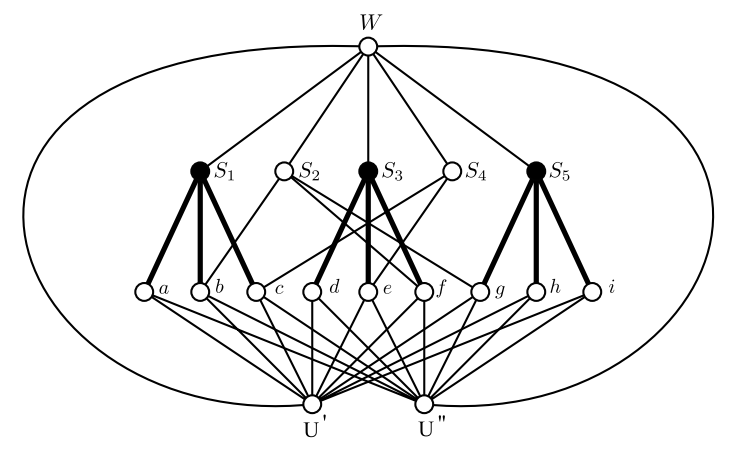
\includegraphics[width=14cm]{img/Figure6-1.png}
\caption{Reduction of Exact Cover by 3-sets to the Minimun Infected Subset. Image source: \cite{Araujo2018}}
\label{fig:reduction}
\end{figure}



\section{Heuristics}
Initial constraints created: the reductions and the one based on the pair of vertices
Initial approach: list all possible S's. Problem 
After, basic greedy heuristic was tried;
Cluster HCS ideia

\section{Instances used and implemented}
Here, describe the coloring problem instances and how instances were build, and the ones based on the paper \citet{raghavan2015}
